\chapter{Proposed Approach}

\section{Prediction Error Sequence Extraction}

In previous work on frame deletion detection in MPEG-2, the prediction error sequence was extracted directly from the video decoder using the DCT coefficients of the prediction error residuals located in the compressed video file. The prediction error was averaged over all macroblocks in a frame. This prediction error was then stored as a sequence. Due to the nature of the correlation between P-frame prediction errors across a single GOP, any prediction made across GOP boundaries would result in increased prediction error \cite{wang}. Wang and Farid showed that for fixed GOP video, the increase in average prediction error is periodic with respect to the number of frames deleted from the video. Stamm's work expands the idea of the prediction error trace by introducing the formulation of the problem as detecting the presence of a fingerprint signal $s(n)$. As H.264 uses variable GOP structures we will only be concerned with the model defined for variable GOP video. Stamm et al. defines the model of $s(n)$ as

\begin{equation}
s(n) = \beta \mathds{1} \left( \Theta(n) = 0 \right).
\label{stammModel}
\end{equation}

where $\beta > 0$ is a constant and $\Theta(n)$ is a random variable distributed over the set $\{0, 1\}$ \cite{stamm}. This model corresponds to modeling the fingerprint signal as randomly occurring sequence of discrete impulses with a magnitude of $\beta$. From this model they pose the detection of frame deletion as distinguishing between two hypotheses:

\begin{equation}
\begin{aligned}
  H_{0} : e(n) &= e_{1}(n). \\
  H_{1} : e(n) &= e_{2}(n) = e_{1}(n) + s(n)e_{1}(n).
\end{aligned}
\end{equation}

Thus, detection of frame deletion is detection of the presence of the modulated fingerprint signal $s(n)e_{1}(n)$. Given an unknown video, Stamm et al. first makes an approximation of the unaltered P-frame prediction error sequence. To do this they use a median filter with a filter width of 3.

\begin{equation}
\hat{e}(n) = \text{median}\{ e(n-1), e(n), e(n+1) \}.
\end{equation}

Thus, the relationship between the estimate and $e_{1}(n)$ is

\begin{equation}
e_{1}(n) = \hat{e}(n) + \epsilon(n).
\end{equation}

where $\epsilon(n)$ is a zero mean random variable representing estimation error.

Using the estimate of the unaltered P-frame prediction error sequence, Stamm et al. calculates $\hat{s}(n)$, which is an estimate of the fingerprint signal modulated by the prediction error sequence as defined by

\begin{equation}
\hat{s}(n) = \text{max}(e(n) - \hat{e}(n), 0).
\label{estfpsig}
\end{equation}

The estimate of the fingerprint signal is floored at 0, as the model of the $s(n)$ dictates that it must be greater than or equal to 0. This estimate of the fingerprint signal can be used to build a detector. The decision function found by Stamm et al. for variable GOP video is

\begin{equation}
\delta_{var} =
\begin{cases}
  H_{0} & \text{if } \frac{1}{N} \sum_{n=1}^{N} \vert \hat{s}(n) \vert < \tau_{var} \\
  H_{1} & \text{if } \frac{1}{N} \sum_{n=1}^{N} \vert \hat{s}(n) \vert \geq \tau_{var}
\end{cases}
\label{origdecision}
\end{equation}

where the decision is made on the basis of the energy in $\hat{s}$.

In MPEG-2, a P-frame is encoded by searching the previous anchor frame for the macroblock which incurs the least error \cite{mpeg2}. This means that the average prediction error for a single P-frame is only asssociated with the previous I or P-frame. H.264 expands the capabilities of its motion compensation and estimation system by allowing prediction from multiple previous frames (and subsequent frames in the case of B-frames) \cite{h264}. If the prediction error trace is extracted via the codec for H.264, the average prediction error associated with one frame is comprised of a linear combination of the average prediction error associated with motion vectors that map to the different anchor frames used in the motion estimation and compensation process. Thus, cross GOP predictions are smoothed out in such a way that it makes the fingerprint energy detector in Stamm et al.'s paper perform inadequately.

To test this, we collected 257 videos from a cell phone camera (the ASUS ZenFone 3 Laser), and generated an altered video with 15 frames removed from the beginning corresponding to each collected video. The encoding parameters were kept constant, and we fixed the GOP of the altered videos to that of the unaltered videos. In this particular case, the GOP structure was 30 frames in length, with 1 I-frame followed by 29 P-frames. We extracted the prediction error sequence directly from the codec, and measured the estimated fingerprint energy as described above.

\begin{figure}[tbp]%
  \centering
  \subfloat[MPEG-2 Detector on MPEG-2]{{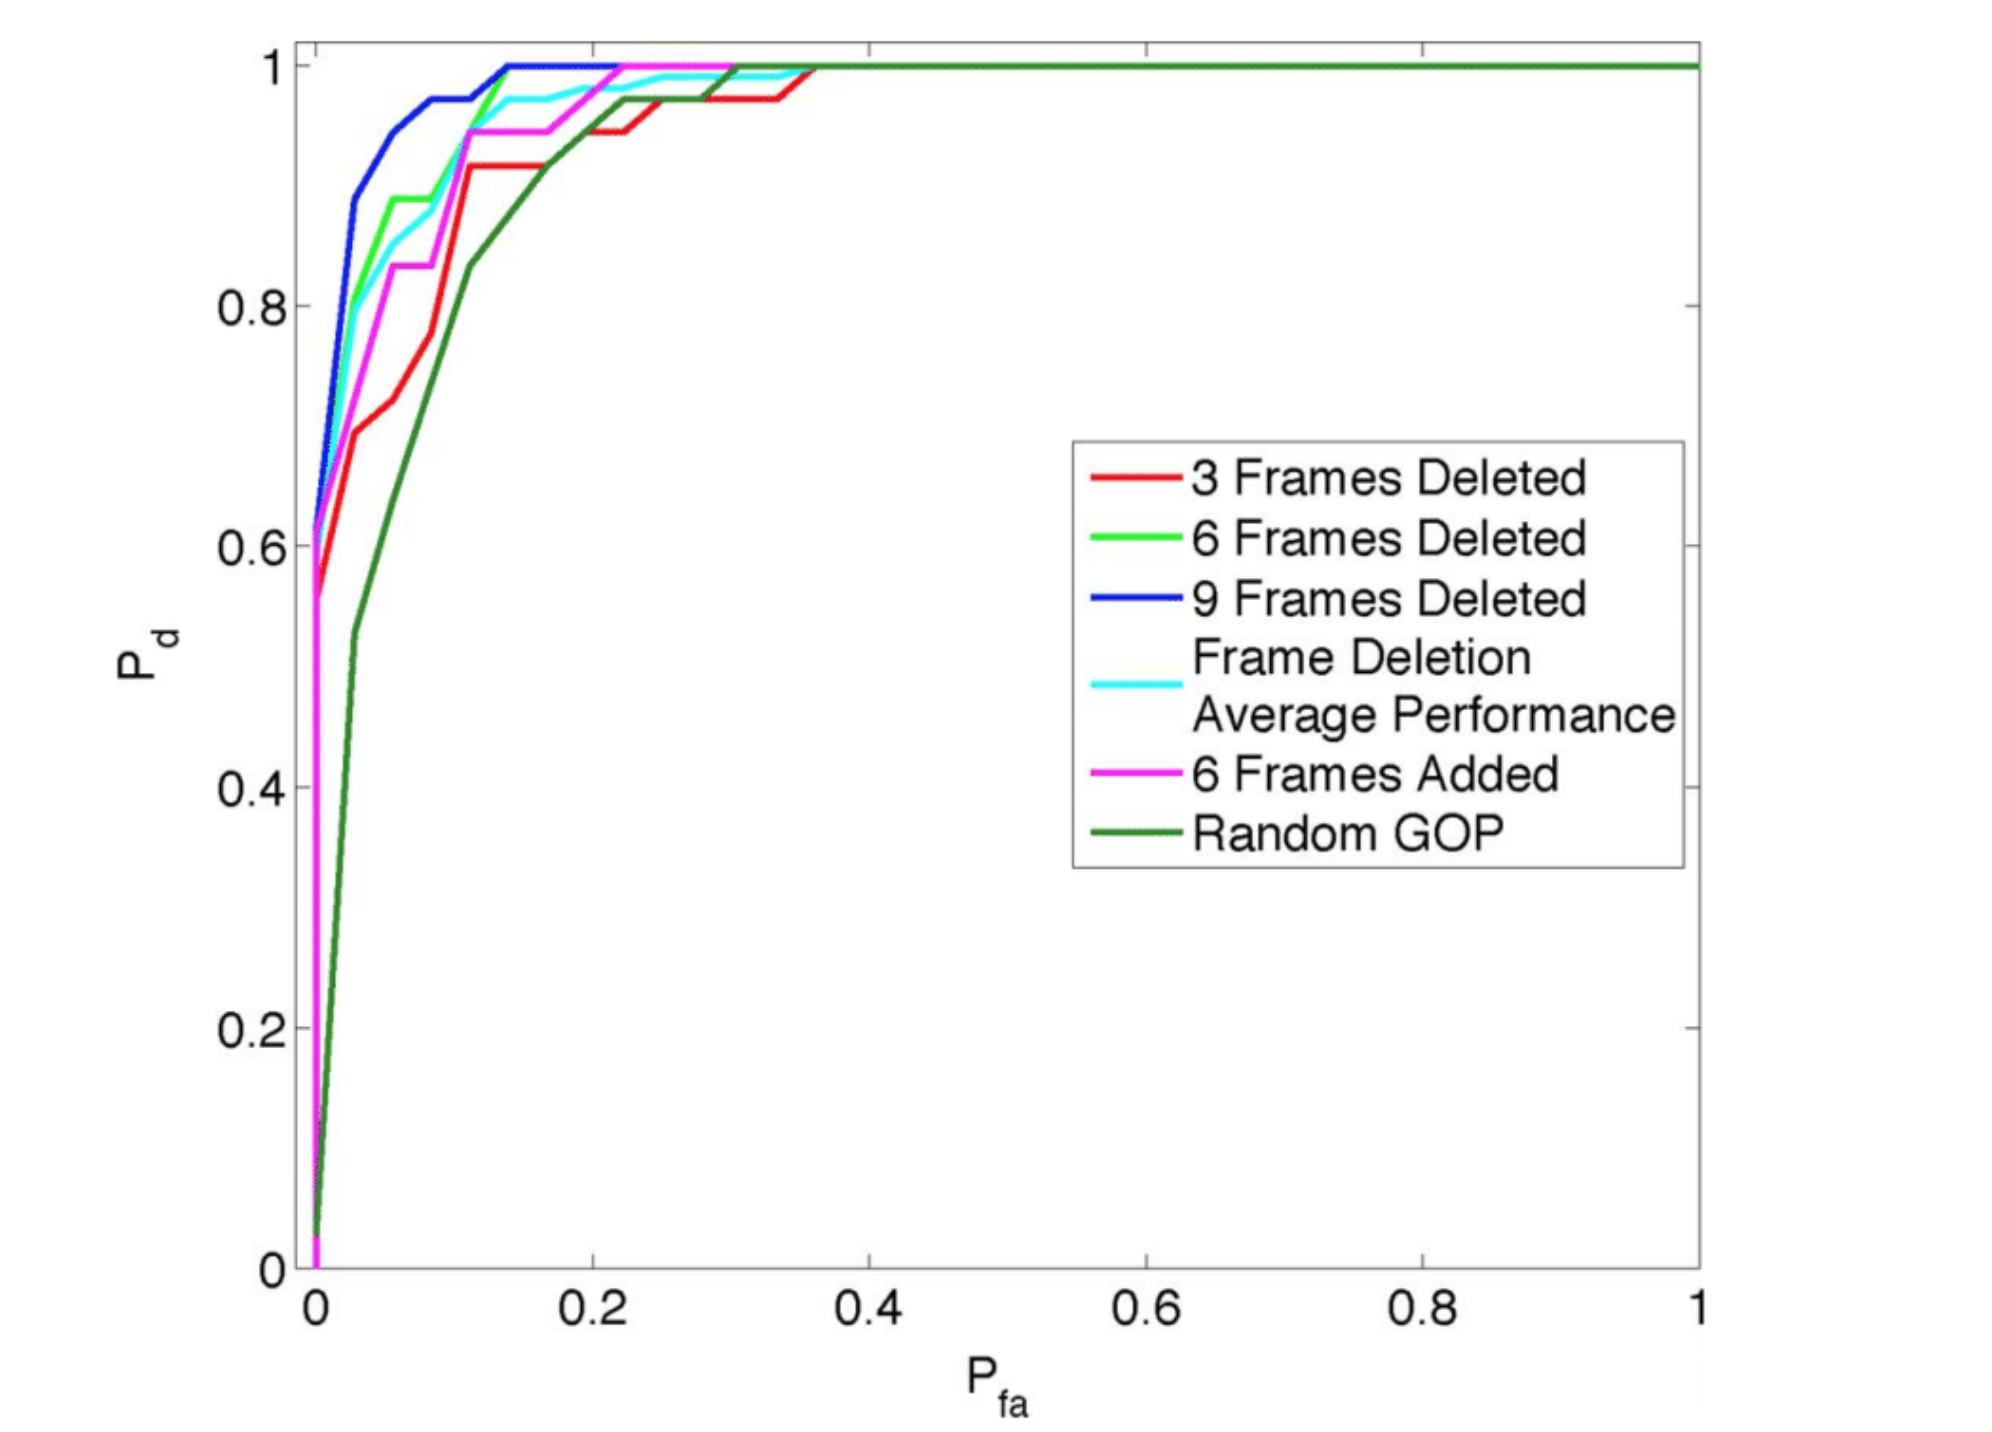
\includegraphics[height=5cm]{ProposedApproach/old_method_roc_mpeg2.png}}}%
  \qquad
  \subfloat[MPEG-2 Detector on H.264]{{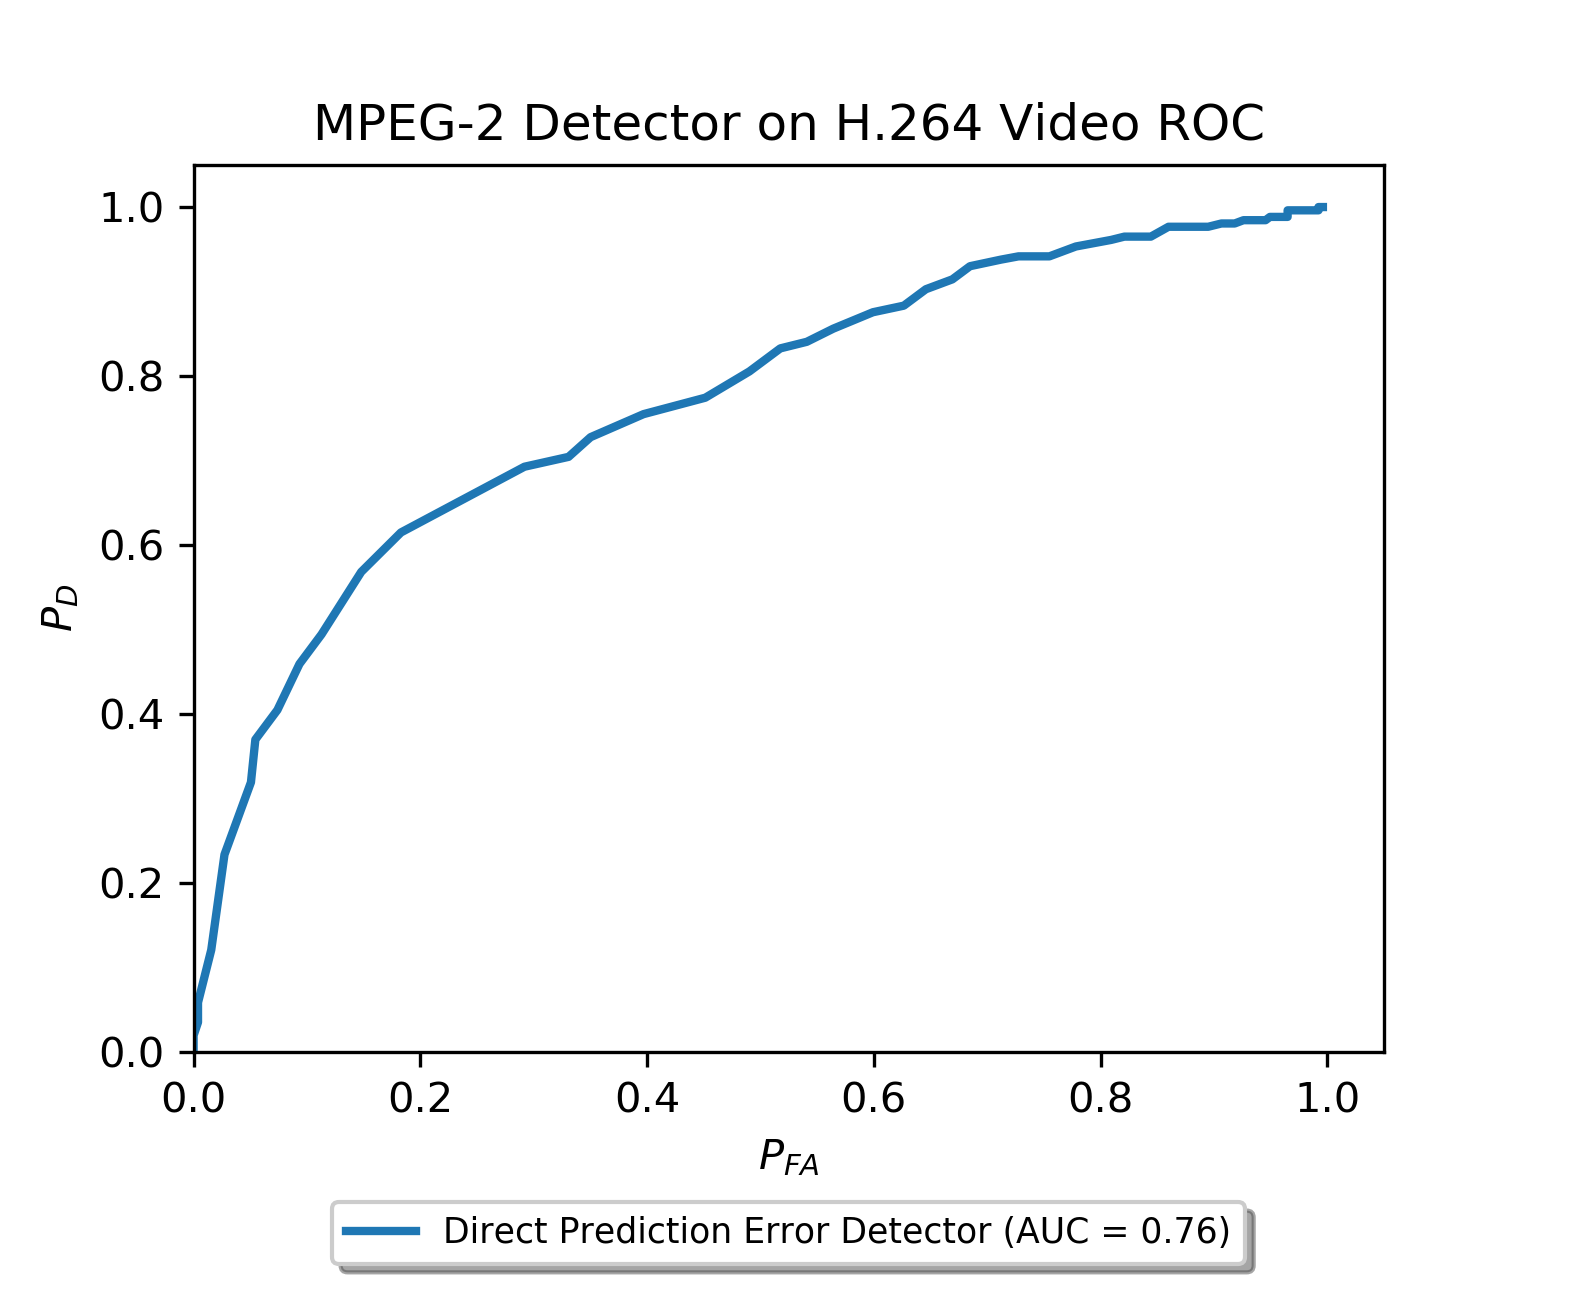
\includegraphics[height=5cm]{ProposedApproach/old_method_roc_h264.png}}}%
\caption[Comparison Between MPEG-2 Detection Methods used on (a) MPEG-2 and (b) H.264]{Comparison Between MPEG-2 Detection Methods used on (a) MPEG-2\footnote{Figure reprinted with permission from Stamm et al.} and (b) H.264}%
\label{oldMethodCompare}%
\end{figure}


As shown in Fig.~\ref{oldMethodCompare} the perfomance of the detector using the methodology derived for MPEG-2 videos suffers a significant decrease when used on H.264 video, particularly at low false alarm rates. This is due to a limitation in the model used by Stamm et al. above in Equation~\ref{stammModel}. As it is possible to predict across multiple previous anchor frames in H.264, the contribution of the fingerprint signal is variable over time. This variation is also not regular, as scene content and motion determine how many cross GOP predictions are present in each P-frame. Thus we propose the updated model for the fingerprint signal as

\begin{equation}
s(n) = \beta(n) \mathds{1} \left( \Theta(n) = 0 \right).
\label{newModel}
\end{equation}

where $\beta(n)$ is now a random variable that takes values in $\R_{\geq 0}$. Thus, we propose the following methodology for extracting the prediction error sequence in H.264.

\subsection{Proposed Prediction Error Sequence Extractor for H.264}

The goal of the proposed extraction algorithm is to maximize the probability that should frame deletion exist, a given measurement of the prediction error comes from a cross-GOP prediction. To this end, instead of directly measuring the prediction error from the DCT coefficients from the decoder, we decode the frame of interest and store the motion vectors associated with said frame. For each motion vector in the current P-frame, we find the x and y coordinates defining the source macroblock which provides the least error mapping from a particular previous anchor frame. Then for that previous anchor frame, we subtract the pixels in the source macroblock from the destination macroblock in the current frame. This leaves us with a prediction error residual associated with the motion vector. We then calculate the average absolute value of this residual.

\begin{figure}[htbp]
\centerline{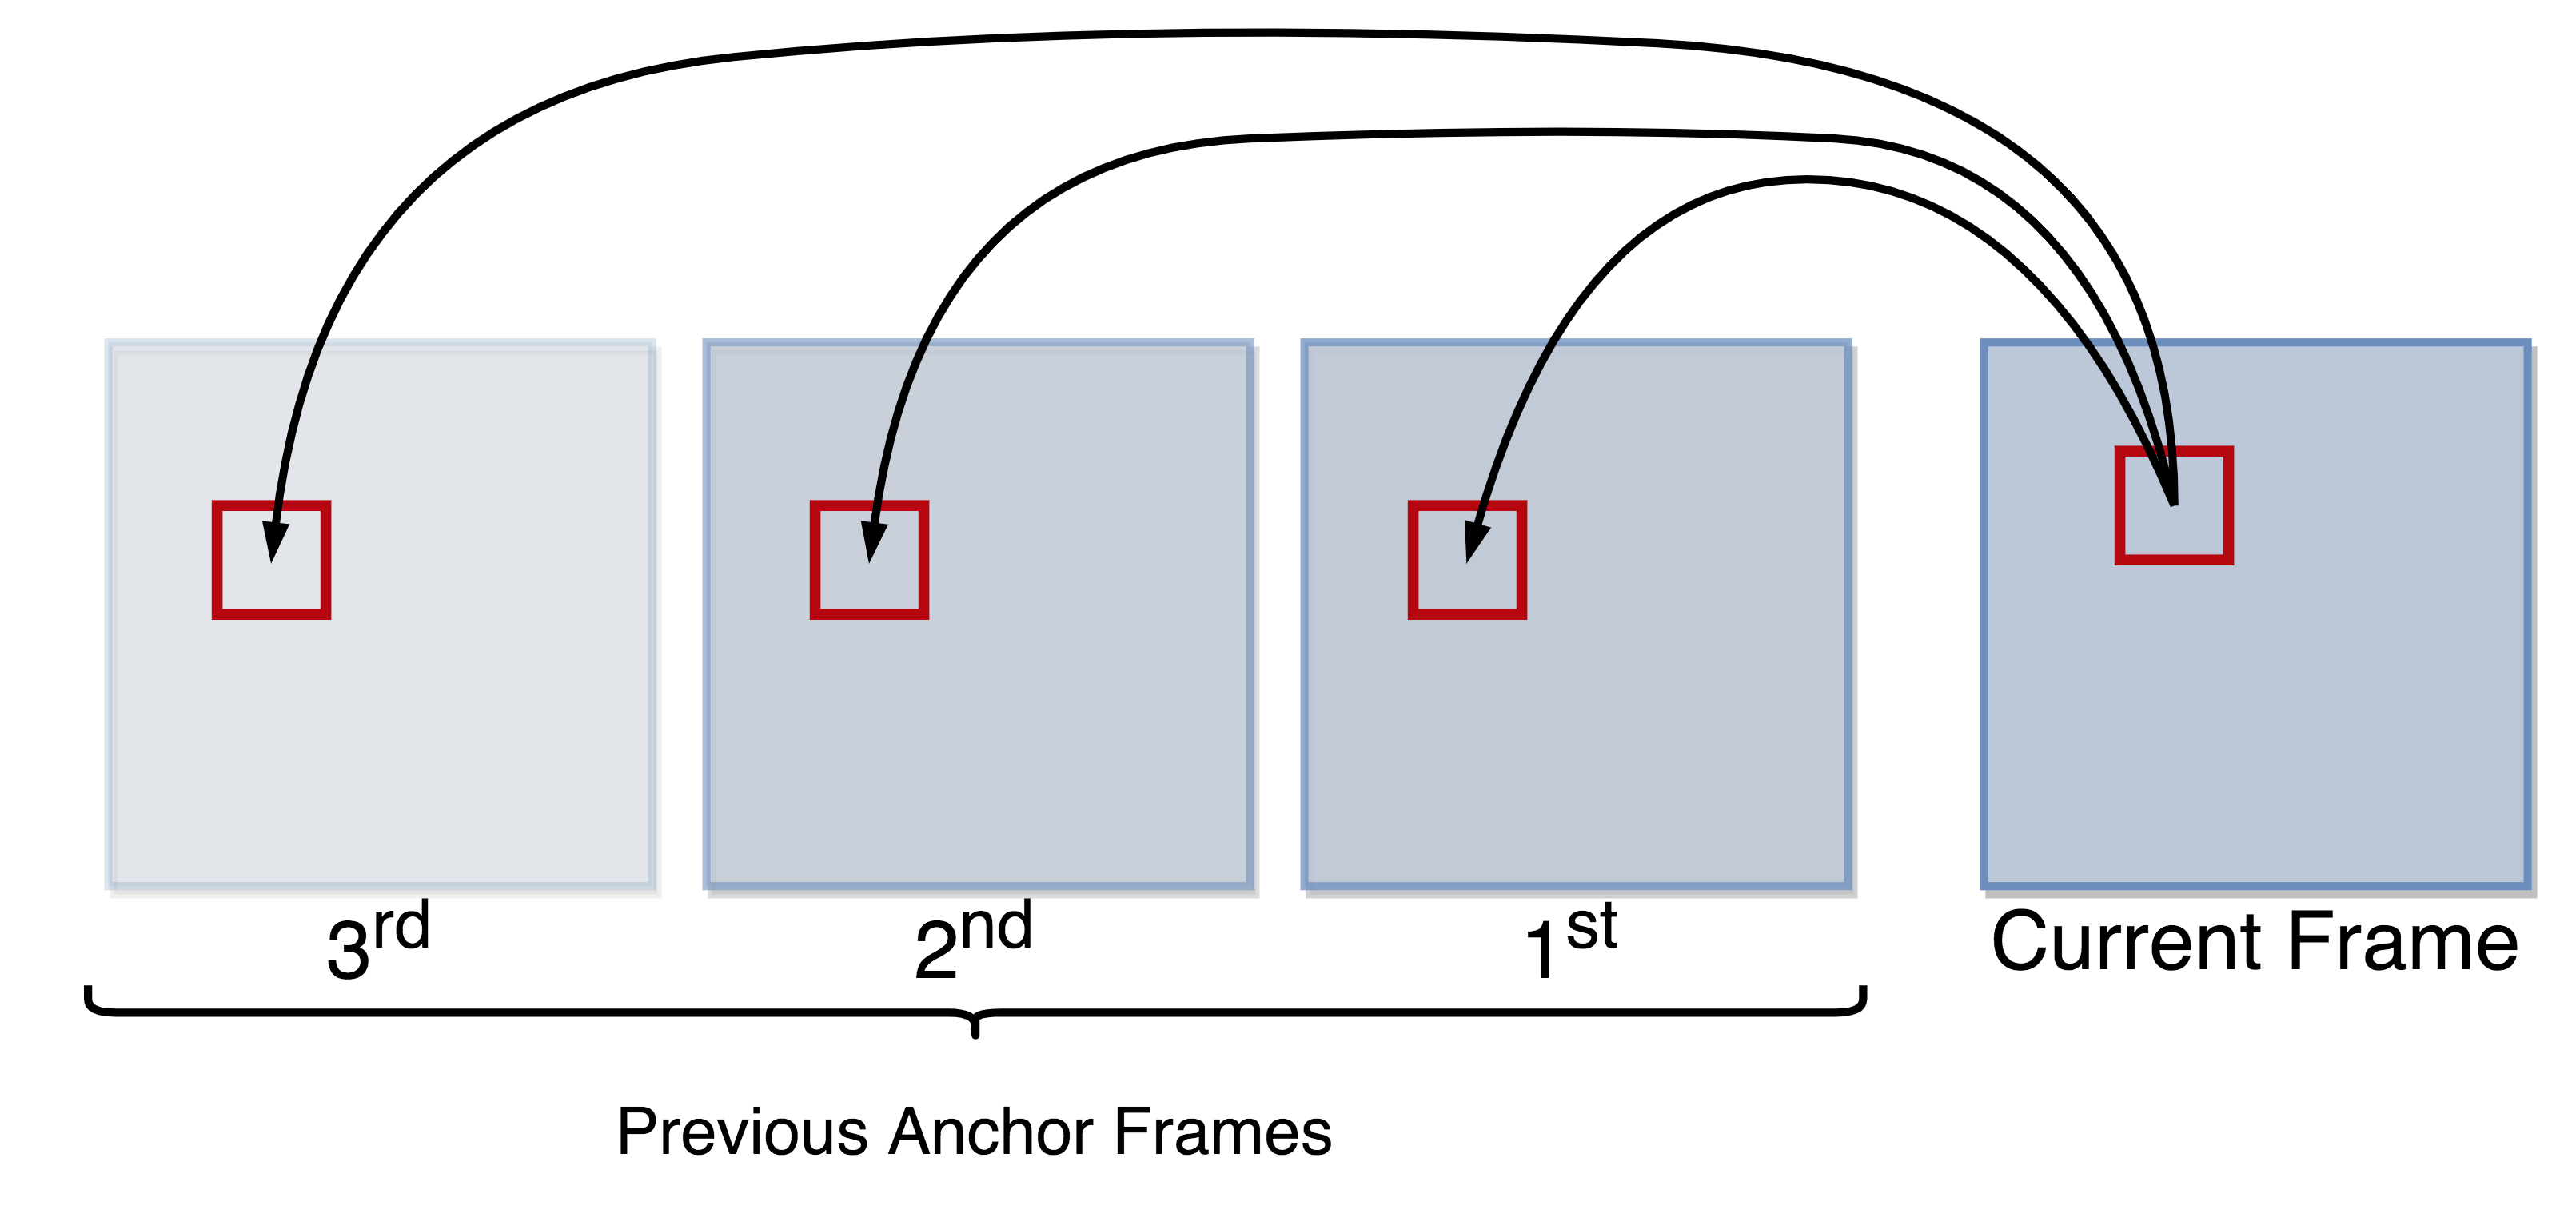
\includegraphics[width=0.9\linewidth]{ProposedApproach/id_source_mb.png}}
\caption{Identification of the source macroblock in 3 previous anchor frames}
\label{srcmbid}
\end{figure}

We repeat this process for each of D previous anchor frames. Then we store these prediction error values in a matrix $M[n]$, where $n$ denotes the P-frame index of the current frame. Each row of the matrix corresponds to the errors associated with a single motion vector, and the columns are the errors associated with each of the previous anchor frames.

After obtaining the $M[n]$ matrix for the current frame, we create the matrix $\tilde{M}[n]$ defined like so:

\begin{equation}
  \tilde{M}_{i, j}[n] = \mathds{1} \left(j = \argmin_{l} \left( M_{i, l}[n] \right) \right) * M_{i, j}[n]
\end{equation}

Thus $\tilde{M}[n]$ is a copy of $M[n]$ where the non-zero entries in each row correspond to the minimum average error associated with the macroblock and all other elements are zero. Effectively, the column index of the non-zero entry is an estimation of which previous frame the motion vector associated with the macroblock maps to in the decoding process.

Further processing is done on $\tilde{M}[n]$ to output only a single prediction error value. First, $\tilde{M}[n]$ is reduced into a vector $P[n]$, such that:

\begin{equation}
  P_{j}[n] = \frac{1}{N_{j}} \sum_{i}{\tilde{M}_{i,j}[n]}
\end{equation}

Where $N_{j}$ is the number of non-zero elements in the $j^{th}$ column of $\tilde{M}[n]$. Then, the reported prediction error for the current frame $e*[n]$ is calculated as

\begin{equation}
  e^{*}[n] = \max_{j} P_{j}[n]
\end{equation}

This entire process is repeated for every P frame in the video. This method of error extraction estimates which previous anchor frame contributes the maximum error per macroblock to the overall prediction error residual obtained by the codec for a given P frame. Since prediction across GOP boundaries results in spikes in the prediction error, the anchor frame that contributes the most error is most likely to be from a different original GOP. In this manner, we obtain a trace that is resilient to advances made in the motion compensation and estimation process in modern codecs as well as robust to variable frame rates and dynamic GOP structures.

\begin{figure}[htbp]
\centerline{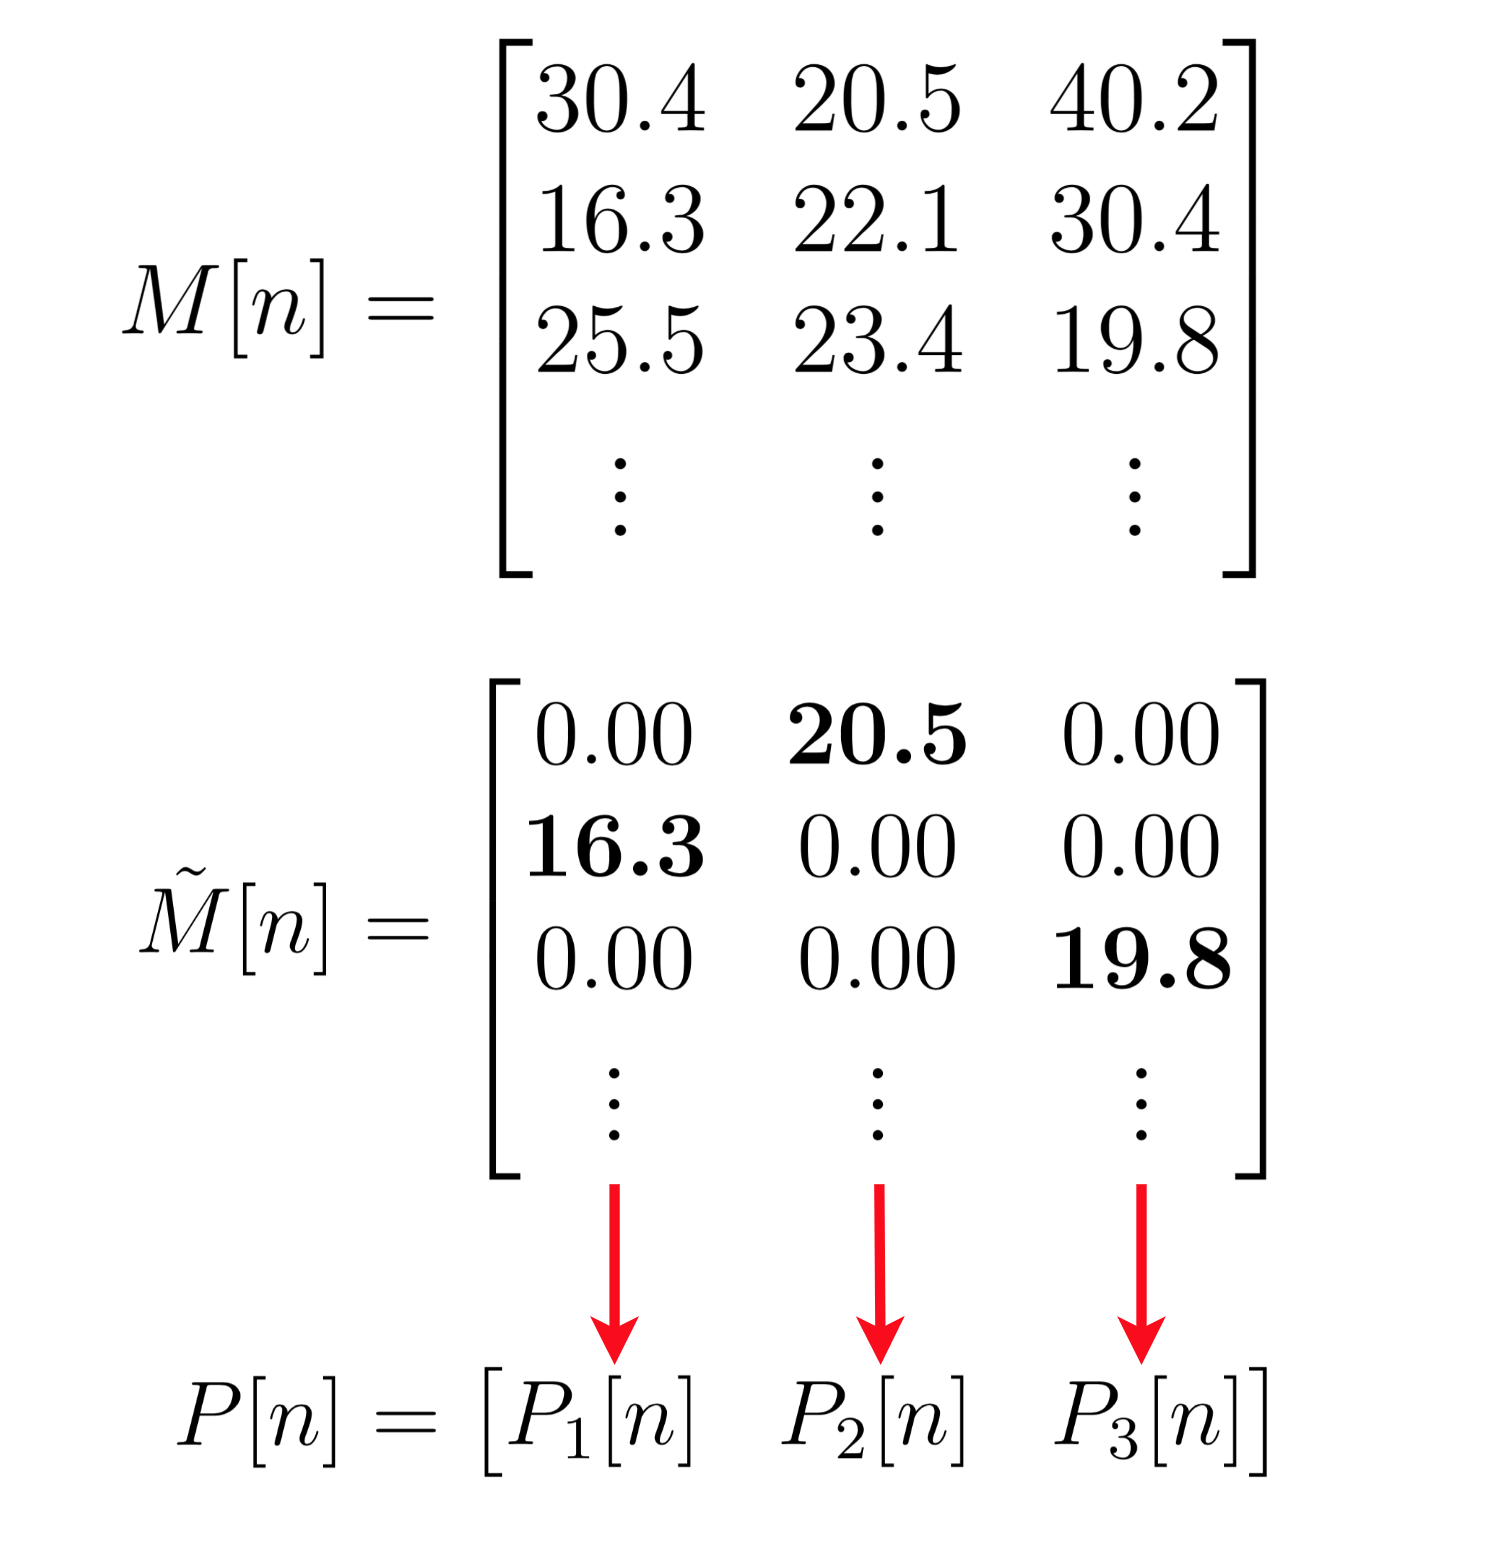
\includegraphics[width=0.55\linewidth]{ProposedApproach/formation_p_vector.png}}
\caption{Methodology for forming $P[n]$}
\label{formp}
\end{figure}

\section{Proposed Detection Algorithm}

In addition to the new methods for prediction error extraction, we propose an expanded detection algorithm to better capture the statistical differences between videos. In fact, depending on scene content, video capture settings, and the amount of motion captured in a single recording, the prediction error sequence and fingerprint signal exhibit different structural behavior. This is true even for videos captured from a single camera model. Figure~\ref{seqCompare} shows this clearly. The two videos were captured from an LG Nexus 5X using the high quality 1080p capture mode. Both videos were shot using similar scene content, but the amount of motion in each video is different. The first video was shot with hight motion, while the second video was comparatively low motion. The top row shows the different prediction error sequences, while the bottom row shows the different estimated fingerprint signals.

\begin{figure}[htbp]
\centerline{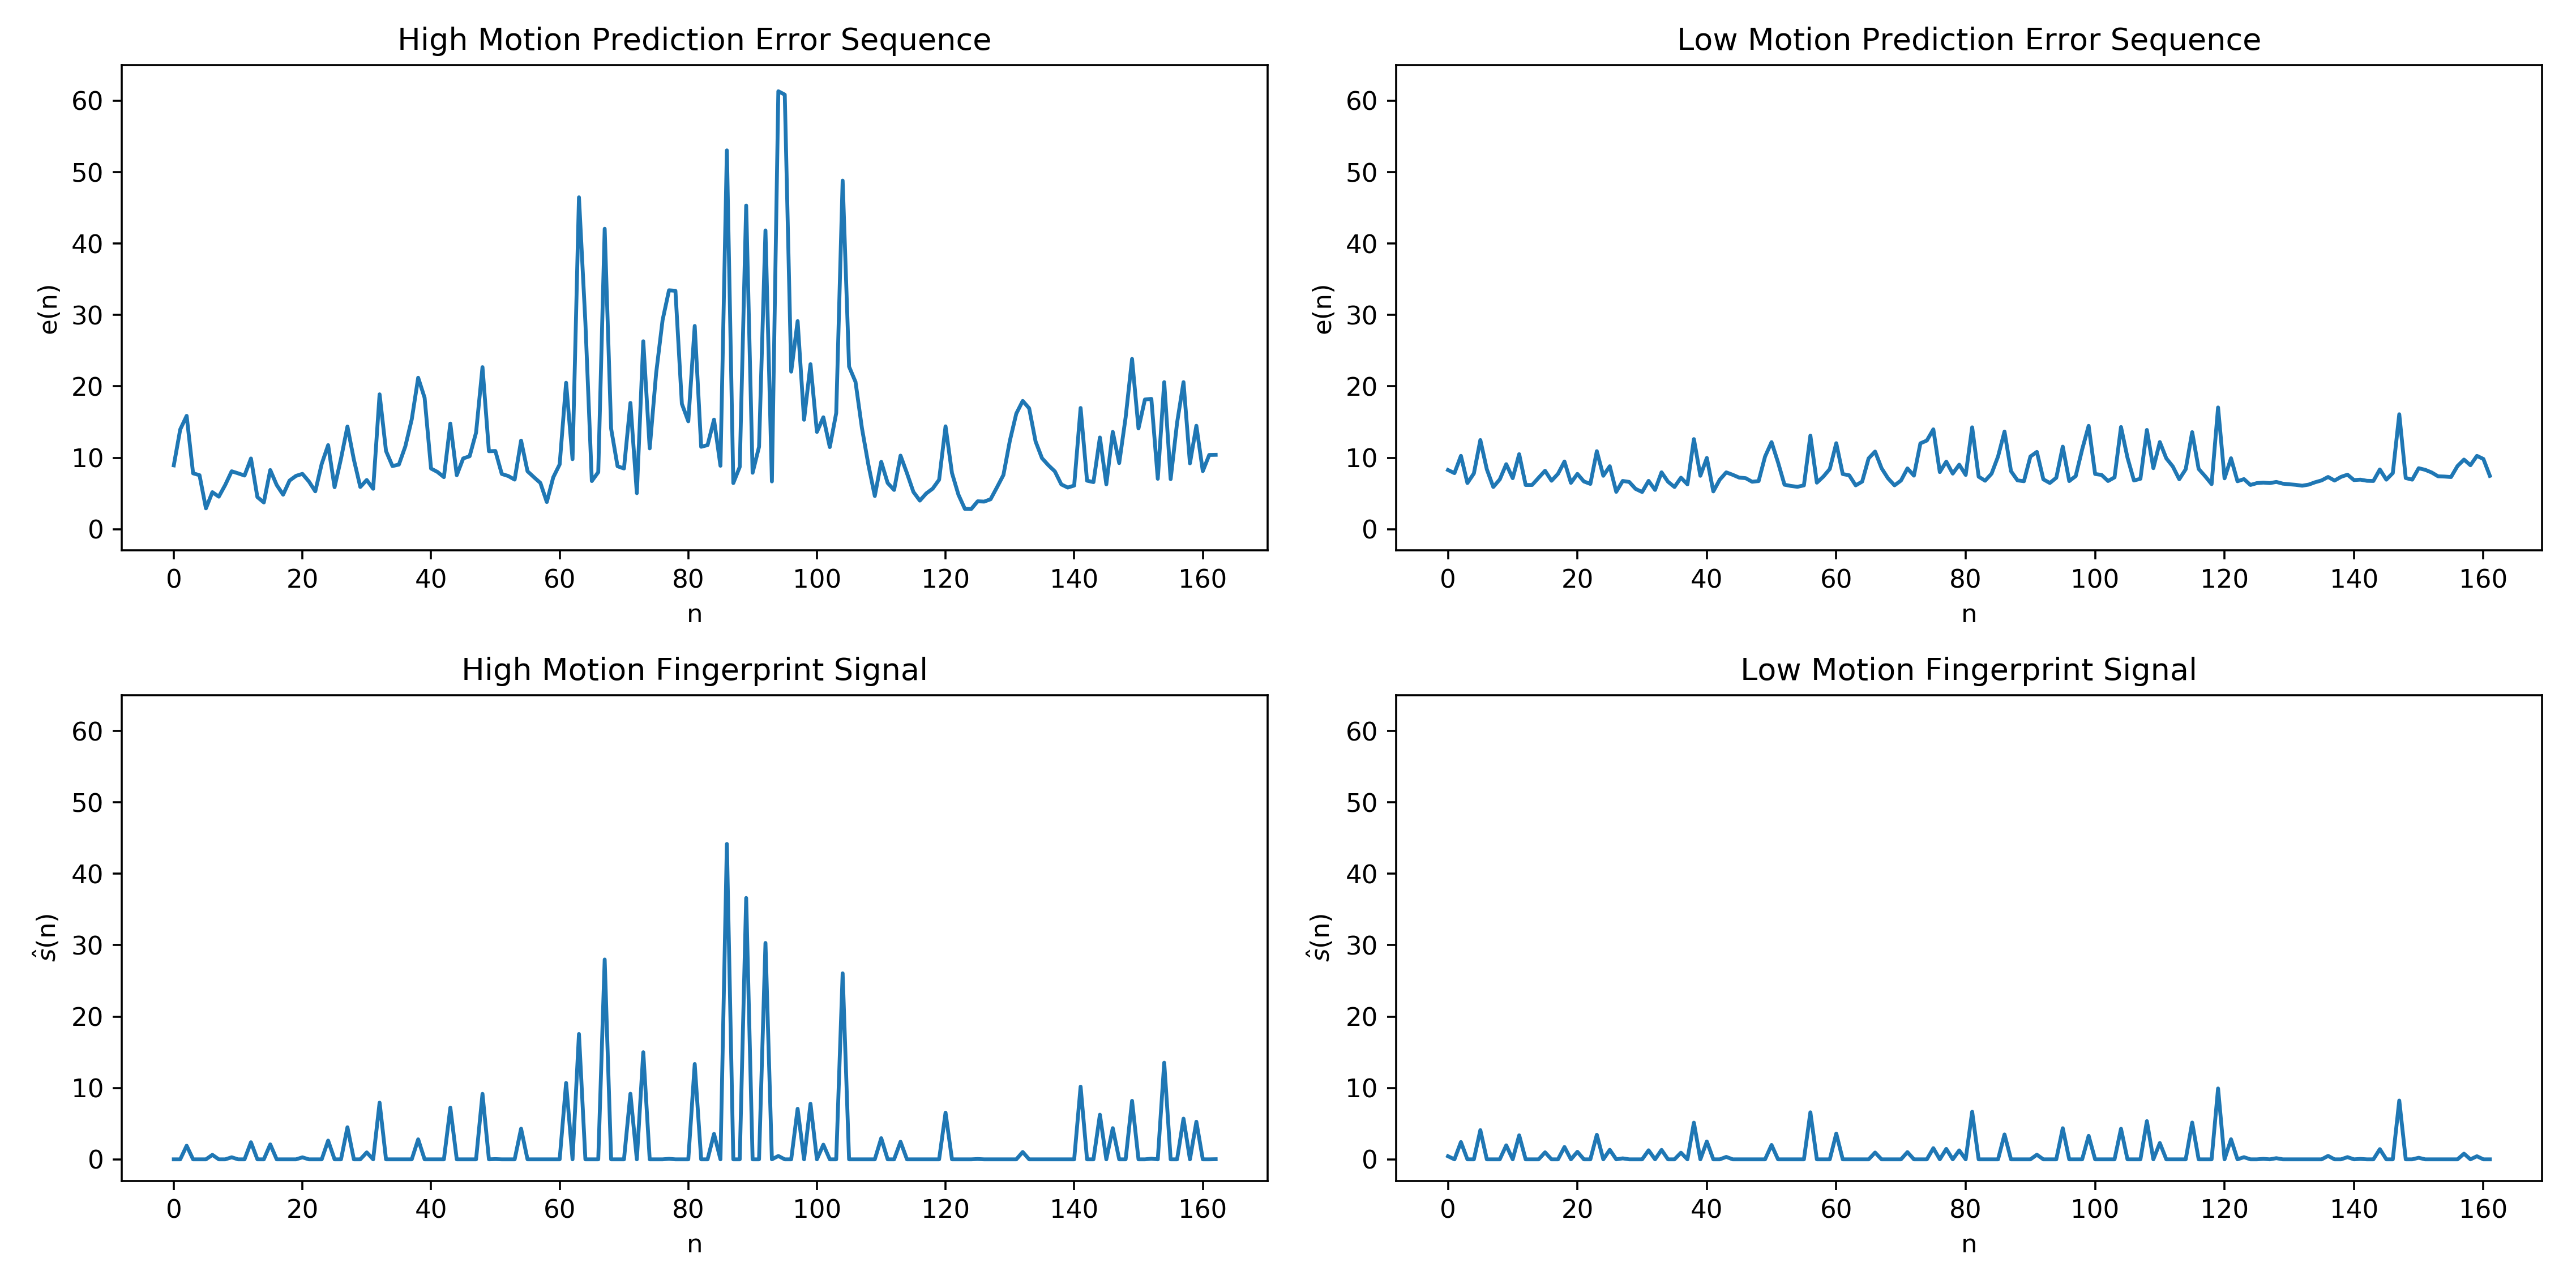
\includegraphics[width=0.9\linewidth]{ProposedApproach/perror_seq_comparisons.png}}
\caption{\emph{Top Left} - The extracted prediction error sequence for a high motion video. \emph{Top Right} - The extracted prediction error sequence for a low motion video. \emph{Bottom Left} - Estimated fingerprint signal for a high motion video. \emph{Bottom Right} - Estimated fingerprint signal for a low motion video.}
\label{seqCompare}
\end{figure}

Notice the large discrepancy in magnitude between both types of signals depending on the amount of motion in the video. The original detection criteria defined by Stamm et al. in Equation~\ref{origdecision} is based on the energy of the estimated fingerprint signal. This will lead to undesirable misclassifications when only using signal energy as the detection feature. Thus, we need a set of new features that can help account for this difference in fingerprint signal energy between videos. 

Under the old model for the fingerprint signal, $\beta$ was a constant, meaning the fingerprint signal was thought of as a randomly occurring sequence of discrete impulses with a magnitude of $\beta$. With the new model defined in Equation~\ref{newModel}, $\beta(n)$ is a random variable that takes nonnegative real values. The effect of $\beta(n)$ can be seen in Fig.~\ref{fdelCompare}. The sample low motion video was reencoded with the first 15 frames removed. This accounts for half of a GOP. As the GOP structure of the video is fixed, it is expected that the fingerprint signal will be periodic \cite{stamm}. The estimated fingerprint signal of the sample video with frame deletion shows some amount of periodicity but the amplitude of the signal varies with time. Modeling this variation of $\beta(n)$ for a given video can help aid in the detection of frame deletion.

\begin{figure}[htbp]
\centerline{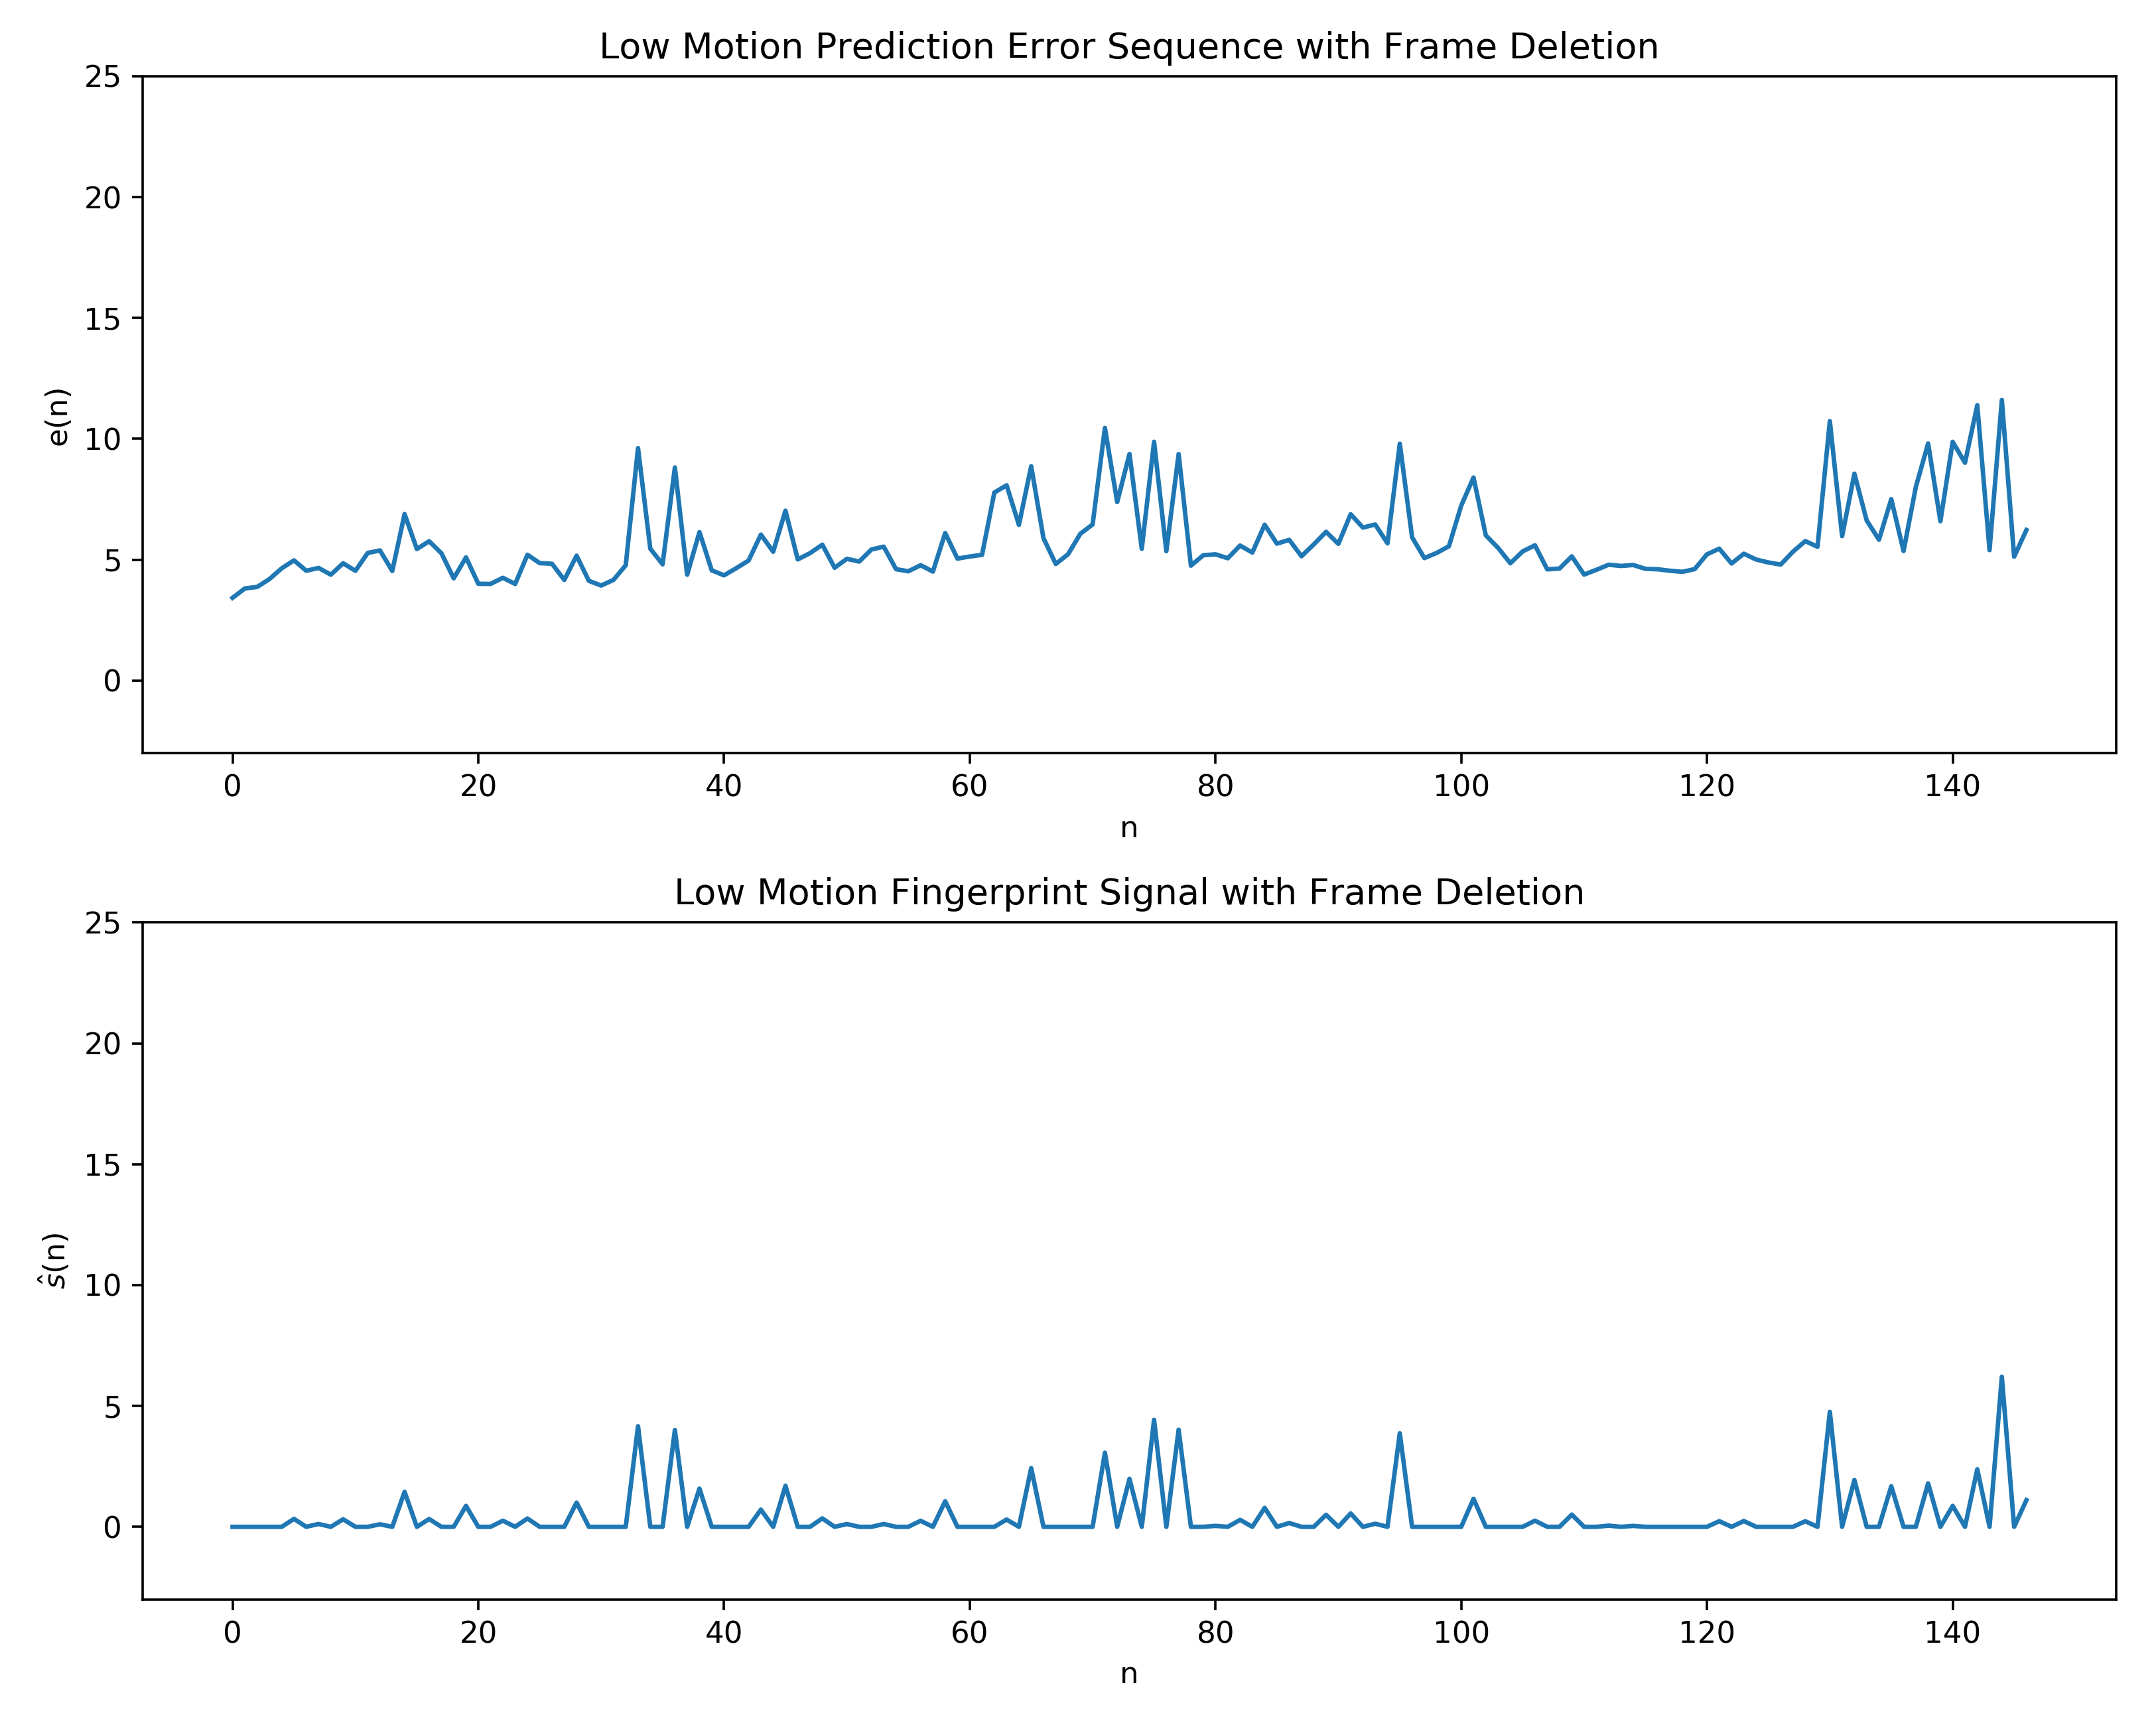
\includegraphics[width=0.75\linewidth]{ProposedApproach/perror_fdel_comparison.png}}
\caption{\emph{Top} - The extracted prediction error sequence for a low motion video with frame deletion. \emph{Bottom} - The Estimated fingerprint signal for a low motion video with frame deletion.}
\label{fdelCompare}
\end{figure}

Over several seconds of video both the prediction error sequence and the fingerprint signal are wide sense stationary. Due to this, we propose modeling both the fingerprint signal and prediction error sequence as autoregressive (AR) processes. The model parameters capture some of the statistical information about $\beta(n)$, and thus are added to a feature vector along with the fingerprint energy. In order to capture the degree to which the model fits a given sequence, the error variance of each AR model is also included. In addition, some basic statistical features are included to scale the overall decision surface. We propose including the mean and variance of both the prediction error sequence and fingerprint signal to the feature vector as well.

For a given video $V$, the feature vector used for classification $\bm{x}_{V}$ is structured as

\begin{equation}
  \bm{x}_{V} = \begin{bmatrix}
    \frac{1}{N} \sum_{n=1}^{N} \vert \hat{s}[n] \vert \\
    \mu_{\hat{s}[n]} \\
    \sigma_{\hat{s}[n]}^{2} \\
    \mu_{e^{*}[n]} \\
    \sigma_{e^{*}[n]}^{2} \\
    \bm{w}_{1} \\
    \bm{w}_{2} \\
  \end{bmatrix}
\end{equation}

Where $\hat{s}[n]$ is the estimated fingerprint sequence of $e^{*}[n]$ obtained by using Equation~\ref{estfpsig} above, but substituting $e^{*}[n]$ for $e[n]$, $\mu$ is the sample mean, $\sigma^{2}$ is the sample variance, $\bm{w}_{1}$ are the $Q^{th}$ order AR model parameters for $e^{*}[n]$, and $\bm{w}_{2}$ are the $Q^{th}$ order AR model parameters for $\hat{s}[n]$.

Note that after creating a feature vector for each video, there is no clear way to make a simple classification. It is inadvisable to create a probabilistic model of the feature vector for classification as there is no clear distribution for the AR model parameters. Instead, we propose using a discriminative function to map an incoming feature vector directly to the set of natural videos or the set of videos altered by frame deletion. As such, we propose using a Support Vector Machine (SVM) classifier with a Radial Basis Kernel function for classification \cite{svm}. 